\documentclass[12pt]{article}
\usepackage{times} 			% use Times New Roman font

\usepackage[margin=1in]{geometry}   % sets 1 inch margins on all sides
\usepackage{hyperref}               % for URL formatting
\usepackage[pdftex]{graphicx}       % So includegraphics will work
\setlength{\parskip}{1em}           % skip 1em between paragraphs
\usepackage{indentfirst}            % indent the first line of each paragraph
\usepackage{datetime}
\usepackage[small, bf]{caption}
\usepackage{listings}               % for code listings
\usepackage{xcolor}                 % for styling code
\usepackage{multirow}
\usepackage{longtable}
\usepackage{float}
%New colors defined below
\definecolor{backcolour}{RGB}{246, 246, 246}   % 0xF6, 0xF6, 0xF6
\definecolor{codegreen}{RGB}{16, 124, 2}       % 0x10, 0x7C, 0x02
\definecolor{codepurple}{RGB}{170, 0, 217}     % 0xAA, 0x00, 0xD9
\definecolor{codered}{RGB}{154, 0, 18}         % 0x9A, 0x00, 0x12

%Code listing style named "gcolabstyle" - matches Google Colab
\lstdefinestyle{gcolabstyle}{
  basicstyle=\ttfamily\small,
  backgroundcolor=\color{backcolour},   
  commentstyle=\itshape\color{codegreen},
  keywordstyle=\color{codepurple},
  stringstyle=\color{codered},
  numberstyle=\ttfamily\footnotesize\color{darkgray}, 
  breakatwhitespace=false,         
  breaklines=true,                 
  captionpos=b,                    
  keepspaces=true,                 
  numbers=left,                    
  numbersep=5pt,                  
  showspaces=false,                
  showstringspaces=false,
  showtabs=false,                  
  tabsize=2
}

\lstset{style=gcolabstyle}      %set gcolabstyle code listing

% to make long URIs break nicely
\makeatletter
\g@addto@macro{\UrlBreaks}{\UrlOrds}
\makeatother

% for fancy page headings
\usepackage{fancyhdr}
\setlength{\headheight}{13.6pt} % to remove fancyhdr warning
\pagestyle{fancy}
\fancyhf{}
\rhead{\small \thepage}
\lhead{\small HW7, Adeniran}  % EDIT THIS, REPLACE # with HW number
\chead{\small CS 532, Spring 2021} 

%-------------------------------------------------------------------------
\begin{document}

\begin{centering}
{\large\textbf{HW 7 - Recommendation Systems}}\\ % EDIT THIS
                                % REPLACE # with HW num and ADD title
Adeniran Adeniyi\\                     % EDIT THIS
DUE Sunday, April 11, 2021 before 11:59pm\\                      % EDIT THIS
\end{centering}

%-------------------------------------------------------------------------

% The * after \section just says to not number the sections
%----------------------------Q1111111111111111111111111111111111

\section*{Q1}
\emph{Find 3 users who are closest to you in terms of age, gender, and occupation.
For each of those 3 users:}
\begin{itemize}
        \item what are their top 3 (favorite) films?
        \item what are their bottom 3 (least favorite) films?
    \end{itemize}
\subsection*{\color{blue}{Answer}}

\lstinputlisting[language=Python,caption=movieLen.py, label=Q1:import,firstnumber=1,firstline=1,lastline=72]{movieLen.py}

% top 3 73
\begin{center}
\begin{longtable}{|l|l|}
\caption{Top 3 movies for user 73} \label{tab:long} \\

\hline  \multicolumn{1}{|c|}{\textbf{Movie Names}} & \multicolumn{1}{|c|}{\textbf{Ratings}}  \\ \hline 
\endfirsthead

\multicolumn{2}{c}%
{{\bfseries \tablename\ \thetable{} -- continued from previous page}} \\
\hline  \multicolumn{1}{|c|}{\textbf{Movie Names}} & \multicolumn{1}{|c|}{\textbf{Ratings}}  \\ \hline 
\endhead

\hline \multicolumn{2}{|c|}{{Continued on next page}} \\ \hline
\endfoot
\hline \hline
\endlastfoot
Three Colors: Red (1994)       & 5.0    \\
Godfather: Part II, The (1974) & 5.0    \\
2001: A Space Odyssey (1968)   & 5.0   
\end{longtable}
\end{center}

%bottom 3 73
\begin{center}
\begin{longtable}{|l|l|}
\caption{Bottom 3 movies for user 73} \label{tab:long} \\

\hline  \multicolumn{1}{|c|}{\textbf{Movie Names}} & \multicolumn{1}{|c|}{\textbf{Ratings}}  \\ \hline 
\endfirsthead

\multicolumn{2}{c}%
{{\bfseries \tablename\ \thetable{} -- continued from previous page}} \\
\hline  \multicolumn{1}{|c|}{\textbf{Movie Names}} & \multicolumn{1}{|c|}{\textbf{Ratings}}  \\ \hline 
\endhead

\hline \multicolumn{2}{|c|}{{Continued on next page}} \\ \hline
\endfoot

\hline \hline
\endlastfoot
Saint, The (1997)   & 2.0    \\
Home Alone 3 (1997) & 1.0    \\
Home Alone (1990)   & 1.0    
\end{longtable}
\end{center}


%user 301 top 3
\begin{center}
\begin{longtable}{|l|l|}
\caption{Top 3 movies for user 301} \label{tab:long} \\

\hline  \multicolumn{1}{|c|}{\textbf{Movie Names}} & \multicolumn{1}{|c|}{\textbf{Ratings}}  \\ \hline 
\endfirsthead

\multicolumn{2}{c}%
{{\bfseries \tablename\ \thetable{} -- continued from previous page}} \\
\hline  \multicolumn{1}{|c|}{\textbf{Movie Names}} & \multicolumn{1}{|c|}{\textbf{Ratings}}  \\ \hline 
\endhead

\hline \multicolumn{2}{|c|}{{Continued on next page}} \\ \hline
\endfoot
\hline \hline
\endlastfoot
It's a Wonderful Life (1946)    & 5.0    \\
Empire Strikes Back, The (1980) & 5.0    \\
Star Wars (1977)                & 5.0    
\end{longtable}
\end{center}


\begin{center}
\begin{longtable}{|l|l|}
\caption{Bottom 3 movies for user 301} \label{tab:long} \\

\hline  \multicolumn{1}{|c|}{\textbf{Movie Names}} & \multicolumn{1}{|c|}{\textbf{Ratings}}  \\ \hline 
\endfirsthead

\multicolumn{2}{c}%
{{\bfseries \tablename\ \thetable{} -- continued from previous page}} \\
\hline  \multicolumn{1}{|c|}{\textbf{Movie Names}} & \multicolumn{1}{|c|}{\textbf{Ratings}}  \\ \hline 
\endhead

\hline \multicolumn{2}{|c|}{{Continued on next page}} \\ \hline
\endfoot

\hline \hline
\endlastfoot
Ready to Wear (Pret-A-Porter) (1994) & 1.0    \\
Dirty Dancing (1987)                 & 1.0    \\
Natural Born Killers (1994)          & 1.0   
\end{longtable}
\end{center}


% user 369
\begin{center}
\begin{longtable}{|l|l|}
\caption{Top 3 movies for user 369} \label{tab:long} \\

\hline  \multicolumn{1}{|c|}{\textbf{Movie Names}} & \multicolumn{1}{|c|}{\textbf{Ratings}}  \\ \hline 
\endfirsthead

\multicolumn{2}{c}%
{{\bfseries \tablename\ \thetable{} -- continued from previous page}} \\
\hline  \multicolumn{1}{|c|}{\textbf{Movie Names}} & \multicolumn{1}{|c|}{\textbf{Ratings}}  \\ \hline 
\endhead

\hline \multicolumn{2}{|c|}{{Continued on next page}} \\ \hline
\endfoot
\hline \hline
\endlastfoot
Dead Poets Society (1989)                               & 5.0    \\
Return of the Jedi (1983)                               & 5.0    \\
Wallace \& Gromit: The Best of Aardman Animation (1996) & 5.0   
\end{longtable}
\end{center}


\begin{center}
\begin{longtable}{|l|l|}
\caption{Bottom 3 movies for user 369} \label{tab:long} \\

\hline  \multicolumn{1}{|c|}{\textbf{Movie Names}} & \multicolumn{1}{|c|}{\textbf{Ratings}}  \\ \hline 
\endfirsthead

\multicolumn{2}{c}%
{{\bfseries \tablename\ \thetable{} -- continued from previous page}} \\
\hline  \multicolumn{1}{|c|}{\textbf{Movie Names}} & \multicolumn{1}{|c|}{\textbf{Ratings}}  \\ \hline 
\endhead

\hline \multicolumn{2}{|c|}{{Continued on next page}} \\ \hline
\endfoot

\hline \hline
\endlastfoot
Beautician and the Beast, The (1997) & 3.0    \\
How to Be a Player (1997)            & 2.0    \\
Booty Call (1997)                    & 2.0   
\end{longtable}
\end{center}

\subsection*{Discussion}
\emph{I created a function called closetToMeAgeGendOccu(),in line 9. This function takes two parameters of the location of u.item and u.data path. u.user was not going through as a parameter so i parsed it directly. From lines 11-27 I read in the datas from each file and store it into dictionary varaibles. In Line 29 -41, I found users that were just as similar to me in age gender and occupation. I limited this search to find only just 3 similar users to me on line 35. These users where stored in a list variable called similarUser. line 31 is the variable declaration, while line 40 appends new users to the list in the created variable\\ \\ Lines 44 to 65, process the outcomes for top 3 movies and bottom 3 movies for each users that I found. Using a for loop to retrieve each user, parse this result to ensure that the said user is in prefs dictionary. If present, retrieve the row of the dictionary of that particular user. Using a pandas dataFrame in Line 51, parse a list of the row item, so that we can easily sort the data based on values in Rating column in descending order. Retrieve the first three data using pandas function .head(3) and the last three data using .tail(3). Save each result as a pandas dataFrame and convert the result to a saved csv file in Q1. \\ \\ \\
My best substitute user is 301, the movies he hates I hate and the movies he enjoys I find them interesting too}

\section*{Q2}
\emph{Which 5 users are most correlated to the substitute you? Which 5 users are least correlated (i.e., negative correlation)?}
\subsection*{\color{blue}{Answer}}
\lstinputlisting[language=Python,caption=question2.py, label=Q2list:import,firstnumber=1,firstline=1,lastline=210]{question2.py}
\begin{figure}[H]
            \centering
            % trim and clip are used to crop the image, trim=left bottom right top
            % width sets max width, height will be scaled appropriately
            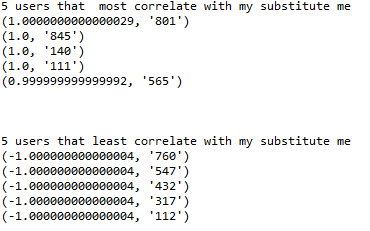
\includegraphics[trim=0 0 0 0, clip, width=\textwidth] {answer.PNG}
            \caption{ The resulting out put for Question 2}
            \label{fig:1}
\end{figure}
\subsection*{Discussion}
\emph{The Final output for the top 5 users that were most correlated to my substitute me were 801,845,140,111, and 565 with their respective correlating score of 1.0000000000000029,1.0,1.0,1.0 and 0.999999999999992. \\ \\ For the bottom 5 users that were most correlated to my substitute me were, 760,547,432,317,and 112. Their correlative score was the same, -1.000000000000004. \\ \\ For the driver lines 139 to 165 generated the resulting output. First I loaded the u.items, u.data and u.user in this function and stored them in a dictionary, dictionary and list variables respectively. I called the topMatches function which I parsed in my substitute me user id in.}


\section*{Q3}
\emph{Compute ratings for all the films that the substitute you has not seen.\\Provide a list of the top 5 recommendations for films that the substitute you should see. \\ \\Provide a list of the bottom 5 recommendations (i.e., films the substitute you is almost certain to hate).}
\subsection*{\color{blue}{Answer}}
Reference question2.py in Listing \ref{Q2list:import}
\begin{figure}[H]
            \centering
            % trim and clip are used to crop the image, trim=left bottom right top
            % width sets max width, height will be scaled appropriately
            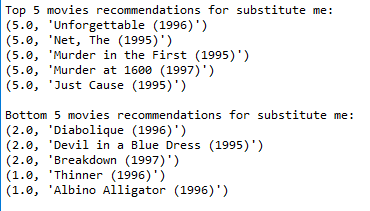
\includegraphics[trim=0 0 0 0, clip, width=\textwidth] {answer3.PNG}
            \caption{ The resulting output for Question 3}
            \label{fig:1}
\end{figure}
\subsection*{Discussion}
\emph{In line 182 to 186, function getRecommendations(prefs,"301") was to get my substiture user recommended list, I Used *recommend[0:5] to get first 5 recommendation. This code was gotten from \url{https://github.com/arthur-e/Programming-Collective-Intelligence/blob/master/chapter2/recommendations.py}\\ 
Top 5 movies recommendations for substitute me, Unforgettable (1996), Net The (1995), Murder in the First (1995), Murder at 1600 (1997), Just Cause (1995)\\ 
Bottom 5 movies recommendations for substitute me,in line 186 *recommend[len(recommend)-5: len(recommend)] used it to extract the bottom 5 movie recommendations for substitute me Diabolique (1996), Devil in a Blue Dress (1995), Breakdown (1997), Thinner (1996), Albino Alligator (1996)}
%\emph{I followed these instruction below:}
\section*{Q4}
\emph{Choose your (the real you, not the substitute you) favorite and least favorite film from the data. For each film, generate a list of the top 5 most correlated and bottom 5 least correlated films.\\
Based on your knowledge of the resulting films, do you agree with the results? In other words, do you personally like/dislike the resulting films?}
\subsection*{\color{blue}{Answer}}
Reference question2.py in Listing \ref{Q2list:import}
\begin{figure}[H]
            \centering
            % trim and clip are used to crop the image, trim=left bottom right top
            % width sets max width, height will be scaled appropriately
            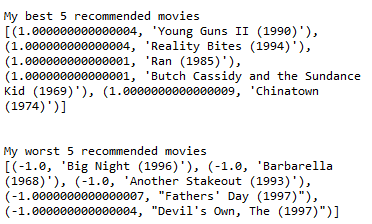
\includegraphics[trim=0 0 0 0, clip, width=\textwidth] {answer4.PNG}
            \caption{ The resulting output for Question 4}
            \label{fig:1}
\end{figure}
\subsection*{Discussion}
\emph{ I first transformed the prefs dictionary to movies. I then selected my best (Vampire in Brooklyn (1995)) movie from the whole list in u.data. The function topMatches and bottomMatch handled the result of the questions 3 \\ \\Top 5 movies recommend from (Vampire in Brooklyn (1995) }
\emph{Young Guns II (1990) \url{https://www.youtube.com/watch?v=r-FmfxLy7fo} I like the movie, a good old movie to me.\\ Reality Bites (1994)  \url{https://www.youtube.com/watch?v=xDYGo0UgIVM} It seem interesting and I would watch it. Just an average movie for me.\\ Ran (1985) \url{https://www.youtube.com/watch?v=YwP_kXyd-Rw} I love this one also, war action my favorite.  \\ Butch Cassidy and the Sundance Kid (1969) \url{https://www.youtube.com/watch?v=YdJW2UxvSFQ} I  do love cow boys like movies\\Chinatown (1974) \url{https://www.youtube.com/watch?v=20FfiP7g4tU} Quite boring but I would enjoy the detective part to movie }

\emph{Worst 5 movies recommended from (Vampire in Brooklyn (1995) \\ \\Big Night (1996) \url{https://www.youtube.com/watch?v=Yd8gK6EgpLM} looks boring to me because its a chef movie\\ Barbarella (1968) \url{https://www.youtube.com/watch?v=M-fJg08wBKw} A complete no to me because its too old and i dont find it interesting at all\\Another Stakeout (1993) \url{https://www.youtube.com/watch?v=Gpm4lGyOVYc} I like this one, action, detective kind of movies\\Fathers’ Day(1997) \url{https://www.youtube.com/watch?v=xsQfKt08Xlk} This kind of movies does not capture my interest at all. Too boring.\\ Devil’s Own, The (1997)\url{Devil’s Own, The (1997) } What I cant believe this is a least favourite movie. I completely love the action in this movie just the first second of seeing it. As usual war movies gets me all the time.]}

\section*{References}
\begin{itemize}
    \item {\url{https://github.com/arthur-e/Programming-Collective-Intelligence/blob/master/chapter2/recommendations.py}}
     \item {\url{https://www.example.com/reallyreallyreally-extra-long-URI/}}
\end{itemize}

\end{document}

